% !TeX root = ../main.tex

\chapter{绪论}

\section{选题意义及选题背景}
随着片上系统(System on Chip,SoC)的发展,越来越多的微处理器和芯片被嵌入到一个
芯片上,导致片上系统的设计复杂性不断提高。在上市时间迅速减少以及功耗降低的需求背景下,
较低抽象层次的RTL设计不能满足SoC设计的需求。现已将设计抽象推向电子系统级别(Electronic System Level,ESL),
能够在SoC设计过程中进行快速原型设计和早期验证\cite{1},或在设计过程能够通过在设计初期能高效迭代探索出比较
准确的设计方向或大致几种比较优秀的方案就显得尤为重要。如果在芯片的RTL设计和验证过程中才发现架构或
软硬件划分无法满足系统功能、性能和成本的要求,就会导致大量的重复工作。ESL设计能够提供比RTL设计更快的仿真速度,
以及根据实际需求所要求的不同抽象层次的时序精度, 以进行SoC系统整体性能的评估。软硬件协同设计采用统一的语言描述
系统功能,可以在实现系统前对整个系统进行仿真,以便于及早发现功能问题。接着根据整个系统的约束对系统进行
硬件划分。然后软件和硬件部分可以同步开发,最后再一起协同验证。采用软硬件协同设计可以大大缩短芯片的开发
周期,并提高芯片性能,降低成本。现如今软硬件协同设计的基本思路如图1.1所示:
\begin{figure}
    \centering
    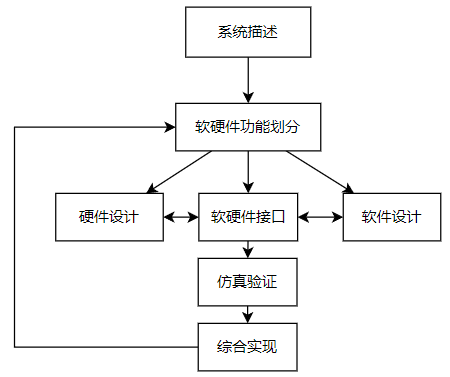
\includegraphics[width=0.5\textwidth]{软硬件协同设计基本思路.png}
    \caption{软硬件协同设计的基本思路}
    \label{fig:badge}
\end{figure}

仿真模型模型的建立和验证是处理器设计周期中一个重要阶段。当前,大多数的处理器仿真模型为C/C++所写,仿
真模型的建立基于SystemC\cite{2}编写,用于统一硬件模型设计以及上层软件平台,这虽然节省了一定的沟通成本,以及
保持体系结构设计及验证阶段模型的一致性。但灵活性较差,为了追求验证结果的精度,系统复杂度较大。因此,
为了较快的完成架构空间探索,我们需要重新设计一个轻量级,且灵活可配置的仿真平台。

在硬件/软件协同设计过程\cite{3}中提高设计生产率的趋势之一是提高抽象水平。如今,大多数设计流程的实现过程都是基
于寄存器传输级别(RTL)的描述。一方面,用于仿真的语言(例如SystemC)提供了更高的抽象级别,另一方面,
通过高层次合成(High Level Synthesis,HLS)\cite{4}的能力也提供了更高的抽象级别。高级综合的目的是双重的。首先,通过在更高层次上描述系
统,可以获得生产率的提高。其次,由于设计转换发生在更高的层次上,因此有更大的探索设计空间的潜力,这将导
致更好的设计。这种发展的重要性直接影响到设计成本。

较大的设计空间、较高的性能目标要求以及紧迫的上市时间要求对系统的设计提出了极大的挑战。通常,设计空间探
索 (DSE)\cite{5} 在早期开发阶段执行,以在满足整体系统设计要求的多个高级设计配置之间进行选择。自动的设计空间中
寻找和探索可行的解决方案。

本仿真设计平台基于Python的Simpy\cite{6}包构建的仿真环境。Python语言具有简易快速的特点,我们可以快速的重构整个
仿真平台。同时基于这种仿真环境构建的仿真平台具有仿真速度快的优点,我们在设计空间探索过程中可以快速进行,
满足设计空间探索的要求。在本文中我们打通了在极大的设计空间中探索能使得系统性能最优的设计参数的设计空间
探索流程。

\section{国内外研究现状及发展趋势}

\subsection{仿真建模技术的发展现状}
随着片上系统系统的复杂度不断提升,高层建模技术由于其更快的建模速度、更短的仿真时间
以及更高的抽象程度逐渐被大多数研发水平高的机构、高校、电子设计自动化(Electronic Design 
Automation,EDA)公司所重视,并开发出多种高水平的仿真模拟工具以及仿真平台,具有代表
性的有Synopsys的CoWare,Mentor的Vista,Carbon的SoC Designer等等。这些工具提供了许多芯片设计
过程中遇到问题的解决方案,从各模块模型的建立、系统架构的分析到功能验证以及时序分析,进一步
分析功耗以及时延等性能指标\cite{38},甚至给出了高层次综合(High Level Synthesis,HLS)方案。

ESL设计作为系统级设计方法,其核心的思想是从算法级模型转变过来的。ESL设计方法学和ESL设计工具
最早是在20世纪90年代提出的。随着SoC设计技术的发展,ESL设计逐渐受到重视,真正能够执行设计
流程的ESL设计工具这些年才出现。ESL设计现在已经发展成系统软硬件设计、协同验证的一种方法学。
ESL设计是以抽象方式来描述SoC系统,给软硬件工程师提供一个虚拟的硬件原型平台,用于进行硬件系统
结构的探察以及软件程序的开发。

现如今硬件建模仿真平台一部分基于C/C++编写,只能进行串行或多线程仿真和验证,后期的硬件原型模型建立需要采
用Verilog等硬件描述语言完成。另外一部分用SystemC完成,SystemC\cite{7}是一种系统级建模语言,
在C++语言的基础上扩展了一系列的硬件库。SystemC更擅长描述
复杂的算法和控制流程,可以更清楚的描述出整个电子系统的复杂行为。SystemC由Accellera定义和推广,SystemC
适用于系统级建模、体系结构探索、性能建模、软件开发功能验证和高级综合,通常和电子系统级设计和事务级建模(TLM,Transaction Level Modeling)
相关联。SystemC语言既能按照硬件设计的要求进行时钟精
确的并行设计,也可以按照软件设计人员的要求进行抽象层级较高的串行设计,还能兼容C语言
、C++语言,且有专门的标准接口处理SystemC语言与硬件语言的连接问题,因此很适合作为桥梁
连接软件设计和硬件设计\cite{37}。SystemC可以在系统级用高级语言同时描述软件
行为和硬件行为,实现软硬件协同设计\cite{40}。图1.2是基于SystemC的软硬件协同设计流程图。

\begin{figure}
    \centering
    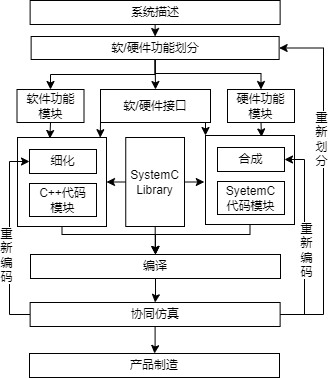
\includegraphics[width=0.5\textwidth]{SystemC软硬件协同设计流程图.png}
    \caption{基于SystemC的软硬件协同设计流程图}
    \label{fig:badge}
\end{figure}

基于SystemC的实现方式相对于前者的优点是仿真平台的建立以及后期硬件模型验证统一起来,能够加快开发流程,节约设计
流程和设计成本。在架构探索阶段,通过对简易建模的仿真分析。得出适合设计要求的架构设计,并在该架构上快速仿真以
得出影响系统性能的因素。在功能验证方面,采用SystemC事务级模型对SoC高层模型进行设计和验证\cite{8}。基于SystemC的标准
事务级建模支持不同系统之间的模型交换。电子系统级设计抽象的描述系统级芯片的行为,能在芯片设计的前期就满足深入
设计芯片系统仿真的需求\cite{9}。这已经成为SoC设计领域前沿的设计方法。

现在又提出了新的仿真工具Simpy,SimPy最初基于Simula和Simscript的思想,但使用标准的Python。它结合了两个以前
的软件包,即Simula风格的SiPy和Simscript风格的SimPy。SimPy 是一个基于标准 Python 以进程为基础的离散事件仿真
框架。SimPy 中的进程是由 Python 生成器构成,生成器的特性可以模拟具有主动性的物件。但现在Simpy很少用于大型平台
建模,主要用于某个具体场景仿真建模即单场景仿真\cite{10},如使用SimPy仿真框架进行基于森林的供应链建模\cite{11}。
\subsection{芯片系统性能分析发展现状}
现如今对于芯片性能进行评估主要从两个方面进行:第一种方法是使用仿真器,如Worm\_sim、NoCSim
、NIRGAM等等。还有一个方法是建立分析模型,如基于排队论或链路拆解原理的分析模型\cite{39}。
前者由于非定制的原因仿真精度不足但仿真速度较快,后者仿真精度高但速度较慢。
现在已经有了能应用于CPU等复杂SoC的仿真工具,如应用广泛的Gem5\cite{12}。它由研究机构和企业合作发展
既支持应用程序仿真又支持全系统仿真,时钟周期准确,可配置并集成工业化标准结构和CPU模型。
\subsection{设计空间探索流程的发展现状}
设计空间探索是指根据系统设计所关心的参数而对不需要的参数进行系统分析和修剪\cite{13},虽然DSE适用于所有类型的系统,但主要
涉及到的还是电子和嵌入式系统。现代嵌入式系统通常具有异构的多处理器系统架构。他们由处理器组成,从完全可编程的内核
到针对时间紧迫任务需求的完全专用的硬件模块。此类系统的组件越来越也多的集成到单个芯片上,从而产生了异构的多处理器
片上系统(MPSoC)架构\cite{14}。为了应对此类系统的复杂性,近15至20年来,电子系统级设计方法这种新设计方法随之出现。并用此
建立里一些高级模型,使建模工作最小化,并对执行速度进行了优化。在此基础上,我们能够在非常早期的设计阶段就应用设计
空间探索。在此探索阶段,可以探索各种不同的设计替代方案。但设计空间探索的过程也极具挑战性,因为探索的设计空间很大。
例如,用于探索应用程序到处理资源的不同映射\cite{15}以及不同调度策略及系统参数对系统性能的影响。

\section{本论文的主要工作}
本文详尽的阐述了一个基于Simpy仿真环境搭建的仿真平台中硬件平台的构建、硬件模型
的建模以及基于这个仿真平台实现的设计空间探索流程。该仿真平台能够快速的让用例在
硬件平台上运行并给出仿真结果及仿真运行过程中的任务执行细节以及硬件资源的利用情
况,打通了设计空间探索的流程,并最终给出设计参数集合的帕累托最优解集。本文将从
以下几个方面进行阐述:

\begin{enumerate}
    \item 仿真平台硬件模块的整体架构设计,主要包括硬件平台配置文件的读取以及根据硬件配置信息实例化硬件IP模型,以及用例文件
    的任务信息的读取及整合,为整个仿真平台的运行打下基础。
    \item 仿真平台Processor模块的整体架构设计,主要是各个硬件模块执行任务的逻辑以及硬件模块的实现,还包括了整个系统中交互
    的基础模型GeneralFifo的实现。
    \item 仿真平台Memory模块的整体架构设计,主要是数据在Memory模块上的读取和存储的逻辑实现,以及Memory模块与总线互联模块的
    交互设计。
    \item 设计空间探索流程的实现,主要包括基于仿真平台实现仿真过程的预测模型,并基于预测模型实现设计空间探索流程,最终给出帕
    累托最优解集,并对设计空间探索结果进行分析。
\end{enumerate}

在整个项目过程中,本人的主要工作如下:

\begin{enumerate}
    \item 设计并实现基于Simpy的仿真平台,完成仿真平台设计中的硬件平台构建模块、
    Processor模块、Memory模块、数据库模块以及整个仿真平台各个模块之间的交互部分。
    \item 根据仿真平台实现预测模型,并基于硬件模块实现设计空间探索流程,并根据最
    终给出的帕累托最优解集给出相应的结果分析。
\end{enumerate}

\section{本文的组织结构}
本文主要分为7个章节,每个章节的具体内容安排如下:

第一章:绪论:介绍不同模型仿真及系统仿真的发展,以及设计空间探索的国内外发展现状,并介绍了本文的研究内容。

第二章:相关技术介绍:对仿真平台及设计空间探索的设计实现所用到的关键技术进行详细的阐述,一方面介绍了系统建模的基础知识
以及我们所采用的仿真环境Simpy框架,另一方面介绍了仿真平台的整体流程以及相关模块的整体设计。

第三章:需求分析:基于仿真平台的功能及性能需求及设计空间探索结果分析准确性的需求的基础上,对仿真平台及设计空间探索的需求
分析进行详细的阐述。

第四章:概要设计:这部分主要是在需求分析的基础上对轻量级仿真平台中硬件平台建模的设计及设计空间探索模块的设计进行简要的阐述,对仿真平台的
整体架构及各个模块的功能划分进行了详细的说明。通过概要设计,为整个应用的实现做好铺垫。

第五章:详细设计与实现:基于概要设计的方案,结合软件工程的的开发思想,详细的介绍了仿真平台硬件平台的搭建、各个硬件模型的
建模、整个用例任务的执行、设计并实现了各个硬件模块之间数据及消息交互相应的接口、设计空间探索流程的具体实现。同时,我们对
设计空间探索流程最终给出的设计参数的集合进行了分析并给出相应的结论。

第六章:系统测试及结果分析:在实现了仿真平台及设计空间探索流程之后,我们基于仿真平台的执行以及结果准确性等方面对整个仿真平
台进行了测试,确保仿真平台能达到预期的结果。

第七章:总结和展望:在本章,笔者对这篇论文进行简单的总结,并对仿真平台及设计空间探索流程中的不足进行了描述,并对仿真平台及
设计空间探索流程提出了未来的展望。

